\documentclass[svgnames]{beamer}

\usetheme{Madrid}
\usecolortheme{seahorse}
\usepackage{multirow}
\usepackage{caption}
\setbeamertemplate{navigation symbols}{}
\useinnertheme{rectangles}

\usepackage{appendixnumberbeamer}
\usepackage[ruled, vlined, longend]{algorithm2e}

\beamertemplatenavigationsymbolsempty
\usepackage[many]{tcolorbox}
\usepackage{color}
\usepackage{varwidth}
\usetikzlibrary{decorations.pathmorphing}
\usetikzlibrary{shadows}
\usetikzlibrary{svg.path}
\usepackage[absolute,overlay]{textpos}

\tikzstyle{cloudconn} = [draw=black, inner sep=0pt,
       line width=0.25mm,{Latex[length=2.5mm, width=1.5mm]}-{Latex[length=2.5mm, width=1.5mm]}]

\tikzstyle{arrowconn} = [draw=black, inner sep=0pt,
       line width=0.25mm,-{Latex[length=2.5mm, width=1.5mm]}]
\makeatother

\usepackage{listings}
\lstset {
  backgroundcolor=\color{white},
  basicstyle=\ttfamily\footnotesize,
  numbers=left,numberstyle=\tiny,numbersep=5pt,
  emph={proc, fun, let, send, consume, global, type, record, if, else,
    in, not, foldt, return, on, ordering, by, as, or },
  emphstyle={\bfseries},
  literate = {=>}{{\bf=>}}2
}
\usepackage{graphicx,accents,pinlabel}
%\useoutertheme{default}
%\useinnertheme{rounded}

\titlegraphic{
\begin{center}
%\includegraphics[width=6cm]{poker_routes}%
\end{center}
}

\usepackage{tikz}
\usetikzlibrary{fadings,shapes.arrows,shadows}
\usetikzlibrary{shadows.blur}
\usetikzlibrary{shapes.symbols}
\usetikzlibrary{backgrounds}
\usetikzlibrary{arrows.meta}
\usetikzlibrary{shapes,snakes}
\usetikzlibrary{fit,calc,shadows}
\usetikzlibrary{arrows,shapes}
\setbeamercolor{section in head/foot}{bg=white, fg=black}
%\beamertemplateshadingbackground{black!10}{blue!15}
\makeatletter
\setbeamertemplate{footline}
{
  \leavevmode%
  \hbox{%
  \begin{beamercolorbox}[wd=.333333\paperwidth,ht=2.25ex,dp=1ex,center]{section in head/foot}%
    \usebeamerfont{author in head/foot}\insertshortauthor~~\beamer@ifempty{\insertshortinstitute}{}{}
  \end{beamercolorbox}%
  \begin{beamercolorbox}[wd=.333333\paperwidth,ht=2.25ex,dp=1ex,center]{section in head/foot}%
    \usebeamerfont{date in head/foot}\insertshortdate{}\hspace*{2em}
  \end{beamercolorbox}%
  \begin{beamercolorbox}[wd=.333333\paperwidth,ht=2.25ex,dp=1ex,right]{section in head/foot}%

    \insertframenumber{} / \inserttotalframenumber\hspace*{2ex} 
  \end{beamercolorbox}}%
  \vskip0pt%
}
\makeatother
\title{Raphytory: big-data temporal graphs}
\titlegraphic{
\begin{center}
\includegraphics[width=3cm]{raphtory_logo}%
\end{center}
}

\author[Raphtory Team] {Raphtory Team (ben@chorograph.com) \\
Presenter Richard G. Clegg} 

\newcommand{\mr}{\mathbb{R}} %math R%
\newcommand{\mn}{\mathbb{N}} %math N%
\newcommand{\mz}{\mathbb{Z}} %math Z%
\newcommand{\bG}{\mathbf{G}}
\newcommand{\bg}{\mathbf{g}}
\newcommand{\btheta}{\mathbf{\theta}}
\newcommand{\var}[1]{\text{var}\left(#1\right)}
\newcommand{\Esym}{\text{E}}
\newcommand{\E}[1]{\Esym\left[#1\right]}
\newcommand{\Probsym}{\mathbb{P}}
\newcommand{\Prob}[1]{\Probsym\left[#1\right]}


\date[Raphtory]{Raphtory, analysing big-data and temporal graphs}

\begin{document}

\frame{

\begin{center}
\Huge{\inserttitle}


\vspace{0.2cm}

\inserttitlegraphic

\vspace{0.2cm}

\scriptsize{\insertauthor}

\vspace{0.2cm}

\scriptsize{\insertdate}

\vspace{0.2cm}

\tiny{(Prepared using \LaTeX \;and beamer.)}
\end{center}
}

\section{Introduction}

\subsection{Introduction}
\definecolor{burntorange}{cmyk}{0,0.52,1,0}
\tikzstyle{superpeers}=[draw,circle,burntorange, left color=\oran,
                       text=violet,minimum width=20pt]

\tikzstyle{big comment} = [draw, fill=blue!40, text=white, text width=8cm, minimum height=0.8cm, rounded corners, drop shadow, align=center]
\def\oran{orange!30}
\tikzstyle{vertex}=[circle,fill=black!25,minimum size=20pt,inner sep=0pt]
\tikzstyle{edge} = [draw,ultra thick,-]

\frame{
\frametitle{A simple introduction to Raphtory}
\begin{block}{What is Raphtory?}
Raphtory allows you to get new insights into your data by viewing it as a ``temporal graph".
\end{block}
\pause
\begin{block}{What is a temporal graph?}
This is a way of looking at how relationships in your data change over time. The next slides will explain.
\end{block}

\begin{center}
\includegraphics[width=3cm]{raphtory_logo}%
\end{center}
}

\frame{
\frametitle{Viewing things as a graph/network}

\centering{
\begin{tikzpicture}[remember picture,auto, thick]
  % Place super peers and connect them
  \foreach \place/\name in {{(0,-1)/a}, {(4,-1)/b}, {(4,2)/c}, {(0,2)/d},
           {(-4,0)/e}}
    \node[superpeers] (\name) at \place {};
  \path <1-3> (a) edge (b);
  \path <1-3> (a) edge (c);
  \path <1-3> (a) edge (d);
  \path <1-3> (a) edge (e);
  \path <1-3> (b) edge (c);
  \path <1-3> (d) edge (e);
  \path <1-3> (c) edge (d);
   %
   % Place normal peers
\node<1>[big comment] at (0,-3){A graph (or network)}; 
\node <2> at (a) {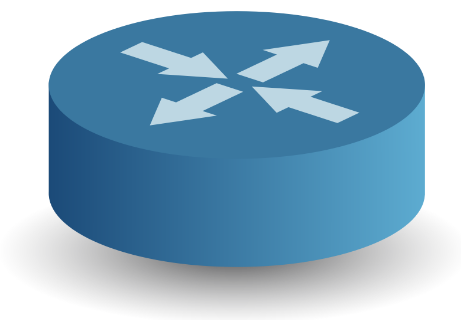
\includegraphics[width=1.2cm]{router}};
\node <2> at (b) {
\includegraphics[width=1.2cm]{server}};
\node <2> at (c) {
\includegraphics[width=1.2cm]{server}};
\node <2> at (d) {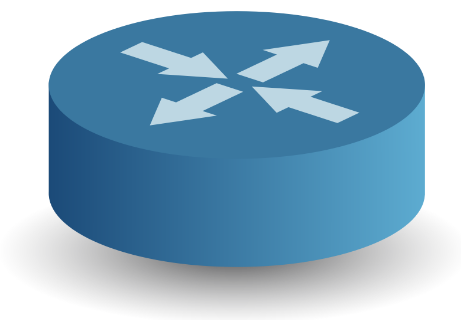
\includegraphics[width=1.2cm]{router}};
\node <2> at (e) {
\includegraphics[width=1.2cm]{server}};
\node<2>[big comment] at (0,-3){A computer network}; 

\path<3>[every node/.style={sloped,anchor=south,auto=false,font=\scriptsize}]
        (a) edge              node {friends with} (b)
        (a) edge              node {friends with} (c)
        (a) edge              node {friends with} (d)
        (a) edge              node {friends with} (e)
        (b) edge              node {friends with} (c)
        (c) edge              node {friends with} (d)
        (d) edge              node {friends with} (e);
\node <3> at (a) {
\includegraphics[width=1.2cm]{redperson}};
\node <3> at (b) {
\includegraphics[width=1.2cm]{blueperson}};
\node <3> at (c) {
\includegraphics[width=1.2cm]{redperson}};
\node <3> at (d) {
\includegraphics[width=1.2cm]{blueperson}};
\node <3> at (e) {
\includegraphics[width=1.2cm]{redperson}};
\node<3>[big comment] at (0,-3){A friendship network}; 

\node <4> (a4) at (a) {
\includegraphics[width=1.2cm]{blueperson}};
\node <4> (b4) at (b) {
\includegraphics[width=1.2cm]{blueperson}};
\node <4> (c4)  at (c) {
\includegraphics[width=1.2cm]{book}};
\node <4> (d4) at (d) {
\includegraphics[width=1.2cm]{book}};
\node <4> (e4) at (e) {
\includegraphics[width=1.2cm]{blueperson}};
\path<4>[every node/.style={sloped,anchor=south,auto=false,font=\scriptsize},
every edge/.style={draw, ultra thick, -{Latex[length=4mm, width=2mm]}}]
        (a4) edge              node {buys} (c4)
        (a4)  edge              node {buys} (d4)
        (b4) edge              node {buys} (c4)
        (e4) edge              node {buys} (d4);
\node<4>[big comment] at (0,-3){A network of purchases};
   %%%%%%%%
   % Legends
\end{tikzpicture}
}
}

\frame{
\frametitle{Graphs are dynamic -- they change}

\tikzstyle{selected edge} = [draw,line width=5pt,-,red!50]
\tikzstyle{selected superpeers}=[draw,red!50,circle, line width= 5pt, burntorange, left color=\oran,text=violet,minimum width=20pt]
\centering{
\begin{tikzpicture}[remember picture,auto, thick]
  % Place super peers and connect them
  \foreach \place/\name in {{(0,-1)/a}, {(4,-1)/b}, {(4,2)/c}, {(0,2)/d},
           {(-4,0)/e}}
    \node[superpeers] (\name) at \place {};
  \path <1-4> (a) edge (b);
  \path <1-4> (a) edge (c);
  \path <1-4> (a) edge (d);
  \path <2> (a) edge [selected edge] (e);
  \path <3-4> (a) edge (e);
  \path <1-4> (b) edge (c);
  \path <1-4> (d) edge (e);
  \path <3> (c) edge [selected edge] (d);
  \path <4> (c) edge (d);
  \node <4> [selected superpeers] (f) at (-4,2) {};
  \path <4> (e) edge [selected edge] (f);
  \path <4> (d) edge [selected edge] (f);

\end{tikzpicture}
}
}

\frame{
    \frametitle{Temporal graphs are important.}
\begin{block}{Why can't we ignore the time dimension?}
The order of events is often vital. We need to know if link A--B happened before the link B--C.
\end{block}
\pause
\centering{
\begin{tikzpicture}%[show background grid]
\draw[white] (-5,-2) rectangle (5,2);
\node <1-> [inner sep=0pt] at (-5,-1) (fc) {
\includegraphics[width=1.3cm]{felix}};
\node <1-> [inner sep=0pt] at (-2.5,0) (ih) {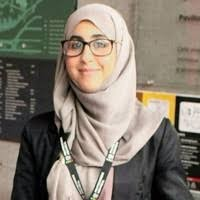
\includegraphics[width=1.3cm]{imane}};
\node <1-> [inner sep=0pt] at (0,.5) (bs) {
\includegraphics[width=1.3cm]{ben}};
\node <1-7> [inner sep=0pt] at (2.5,-0.5) (rc) {
\includegraphics[width=1.3cm]{rich}};
\node <1-> [inner sep=0pt] at (5,1) (na) {
\includegraphics[width=1.3cm]{naomi}};
\node <8-> [inner sep=0pt] at (2.5,-0.5) (rc) {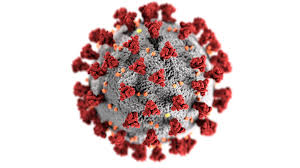
\includegraphics[width=1.6cm]{covid}};
\path[draw] <4-7> (ih) edge[cloudconn] (fc);
\path[draw] <5-7> (ih) edge[cloudconn] (bs);
\path[draw] <6-7> (rc) edge[cloudconn] (na);
\path[draw] <7> (rc) edge[cloudconn] (bs);
\path[draw] <9-> (ih) edge[cloudconn] (fc);
\path[draw] <10-> (ih) edge[cloudconn] (bs);
\path[draw] <11-> (rc) edge[cloudconn] (na);
\path[draw] <12> (rc) edge[cloudconn] (bs);

\end{tikzpicture}
}
}

\frame{
\frametitle{Raphtory design philosophy}
\begin{block}{Time changes are important}
Raphtory is designed to answer questions about time in graphs: Who has contacted John after 1st September? Which product did people buy in the week after they bought product X?
\end{block}
\pause

\begin{block}{Graph data can be large}
Raphtory is designed to be distributed over many computers when a graph is too large to fit within the memory of one computer.
\end{block}
\pause
\begin{block}{Simple to deploy at any scale}
Raphtory is designed to work on a single machine but to be easy to scale to work on dozens of machines in a cloud platform.
\end{block}

}

\frame{
    
\frametitle{Example: Transaction network}

This slide will be an example involving a transaction network showing tracking tainted money
}

\frame{
\frametitle{Current use cases}
\begin{block}{Financial networks}
Analysing transaction networks (bitcoin) to identify fraud and ``dark markets" where illegal transactions happen. 
\end{block}

\begin{block}{Online social networks}
Analysing user interactions (the Gab network) to identify when important users rise to fame.
\end{block}

\begin{block}{Transport networks}
Analysing how users move through cities using public and private transport and how this can be influenced.
\end{block}

}

\frame{
    \frametitle{Other graph technologies}
    
}

\frame{
\frametitle{Finding out more about Raphtory}
    
}

\end{document}
